\documentclass{article}
\usepackage{latexsym}
\usepackage{graphicx}
\usepackage[squaren,Gray]{SIunits}
%\usepackage{SIunits}
\usepackage{mhchem}
%\usepackage{subfigure}
%\usepackage{fullpage}

\title{Calorimeter R\&D}

\begin{document}
\maketitle

\section{SDHCAL - Micromegas calorimetry}
\subsection{Introduction}
The Micromegas R\&D is primarily intended for Particle Flow calorimetry at future linear colliders. It focuses on hadron calorimetry with large-area Micromegas segmented in very small readout cells of $1\times\unit{1}{cm^{2}}$. This granularity provides unprecedented imaging capability which can be exploited to improve the measurement of jet energy.

After construction and test in beam of 4 large-area prototypes of $1\times\unit{1}{m^{2}}$, R\&D efforts were deployed to suppress sparking by means of resistive electrodes. Spark suppression was experimentally demonstrated with different electrode configurations in 2013. Charge-up of the resistive electrodes and resulting gas gain (and efficiency) loss were measured and seen to obey the Ohmic law. In the last 2 years (2014-2015), a particular electrode configuration was optimised for maximal rate capability and full spark suppression. Several Micromegas prototypes with a resistivity varying over 5 orders of magnitude were constructed. A systematic study of sparking and rate capability was then carried out. Results indicate a threshold resistivity above which sparking is suppressed while charge-up effects are small.



\subsection{Recent Milestones}

\subsubsection{A model of spark quenching in resistive Micromegas}
\label{quench_model}

The optimisation of resistive Micromegas for spark suppression and high-rate capability requires some understanding of the underlying charge-up mechanism. Upon irradiation, the potential of the resistive anode surface will change according to its capacitance to ground. At the same time, the surface charge will flow through the bulk to ground: the potential decreases in time, following the RC time constant of the circuit. The time constant indicates the threshold rate above which the gas gain is reduced, namely the rate capability.

During the development of a spark, several single-electrons are multiplied by avalanche in a small region of the amplification gap.
These electrons may originate from photon-feedback at the mesh or from the drift region where they are released during the absorption of a highly ionising particle (\textit{e.g.} an alpha particle). If the time between avalanches is shorther than the RC time constant, the film can be treated as an insulator. Its surface will charge-up according to the avalanche current density. This will result in a progressive reduction of the electric field and a quench of the spark at an early stage of development.

\subsubsection{Resitive prototype design}

The charge-up model predicts that sparking should be suppressed if the RC constant is longer than the avalanche time-scale.
To test the validity of the model, a systematic study was conducted using prototypes of different RC constant.
Each prototype is a square matrix of 10$\times$10 square readout pads of 1$\times$\unit{1}{cm^{2}}.
Each pad is then dressed with a resistive electrode consisting of a resistive pad and an embedded resistor (Figure~\ref{embeddedR}).
The RC constant is controlled by the pattern and resistivity of the embedded resistor.
Three patterns were considered to vary the time constant over 3 orders of magnitude.
A first batch of 3 prototypes was built in 2014 with a resistivity of \unit{100}{kOhm/\Box}.
In 2015, another batch of 3 was built with a resistivity of \unit{1}{kOhm/\Box}.
The estimated RC range available for test lies between \unit{1-10}{ns} and \unit{10-100}{\micro s}.
Non-resistive prototypes were also built for reference.


\begin{figure}[h]
\begin{centering}
  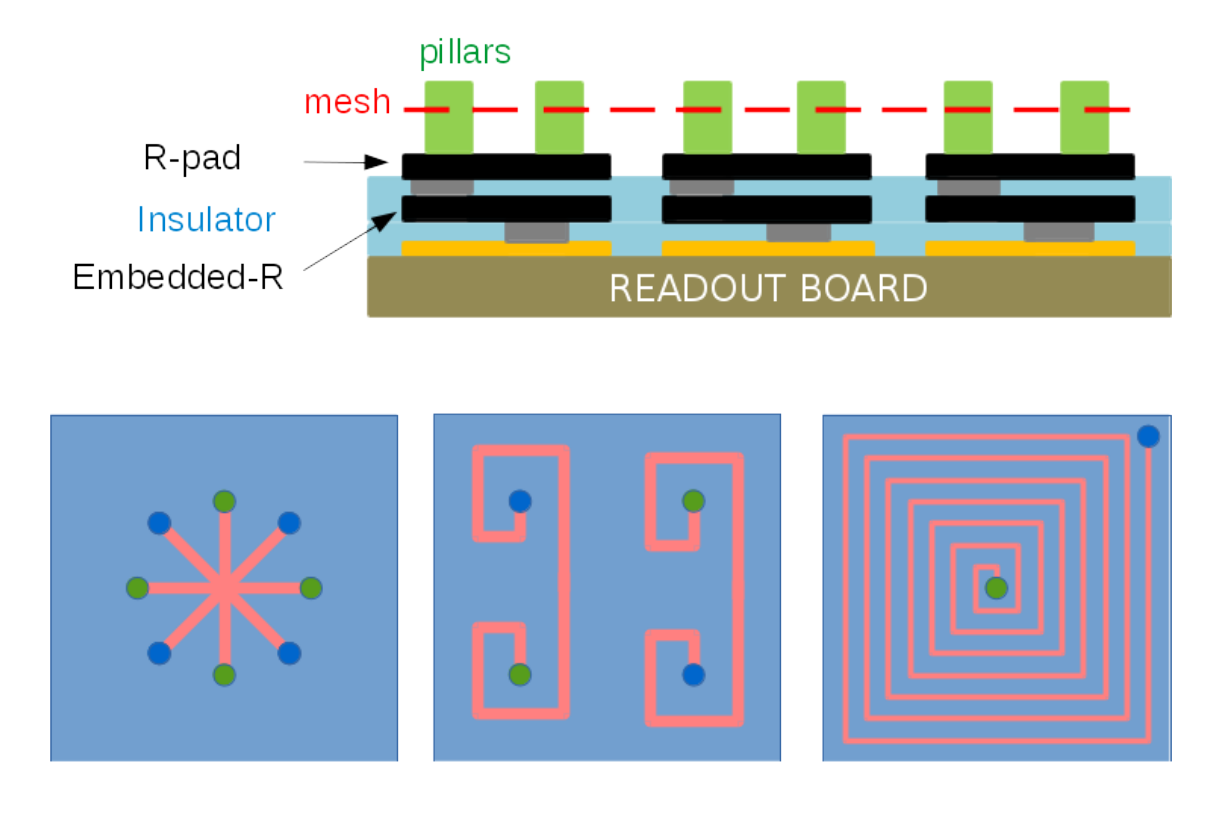
\includegraphics[width=0.55\textwidth]{embeddedR}
  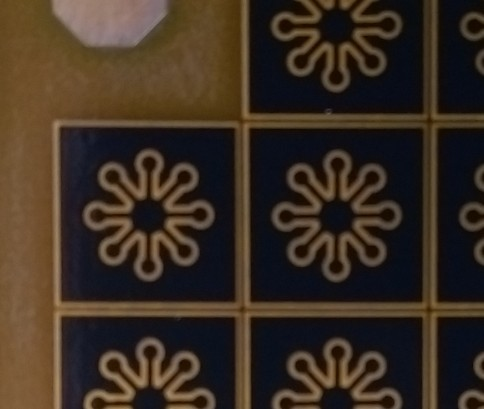
\includegraphics[width=0.4\textwidth]{star_pattern}
  \caption{Electrode configuration: resistive pad and readout pad are connected by an embedded resistor (left). On the right: photograph of one corner of a pad board showing the embedded resistors prior to the serigraphy of the resistive pads and the lamination of the Bulk mesh.}
\label{embeddedR}
\end{centering}
\end{figure}


\subsubsection{Rate capability}

The rate capability was assessed using an \unit{8}{keV} X-ray beam collimated to an 8\,mm$^{2}$ diameter spot on the detector window. After calibration of the event rate with a non-resistive prototype operated in pulse-counting mode, the current through the resistive prototypes was measured as a function of rate.
The current-response of 2 resistive prototypes, measured at different values of gas gain, is shown in Figure\,\ref{rateCapa}.
Above a certain rate, the response of the two prototypes deviates from linearity as a result of charging-up of the irradiated resistive pad.
The figure also shows that charge-up effects become more pronounced with increasing rate, gas gain and resistance, as expected from the Ohmic law.
At intermediate RC values (\unit{0.1-1}{\micro s}) (Figure\,\ref{rateCapa} (left)) and at a working gain around 4000, charge-up effects are negligible up to a rate of \unit{1}{MHz/mm^{2}}. At a rate of \unit{10}{MHz/mm^{2}}, the relative gas gain loss is roughly 25\,\%.

\begin{figure}[h]
\begin{centering}
  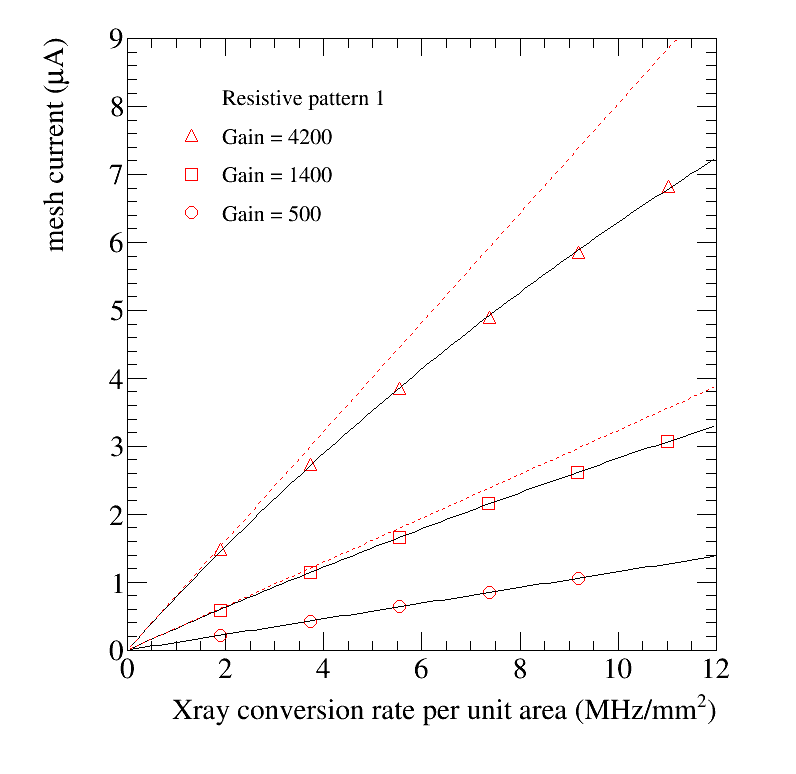
\includegraphics[width=0.45\textwidth]{imesh_rate_star} 
  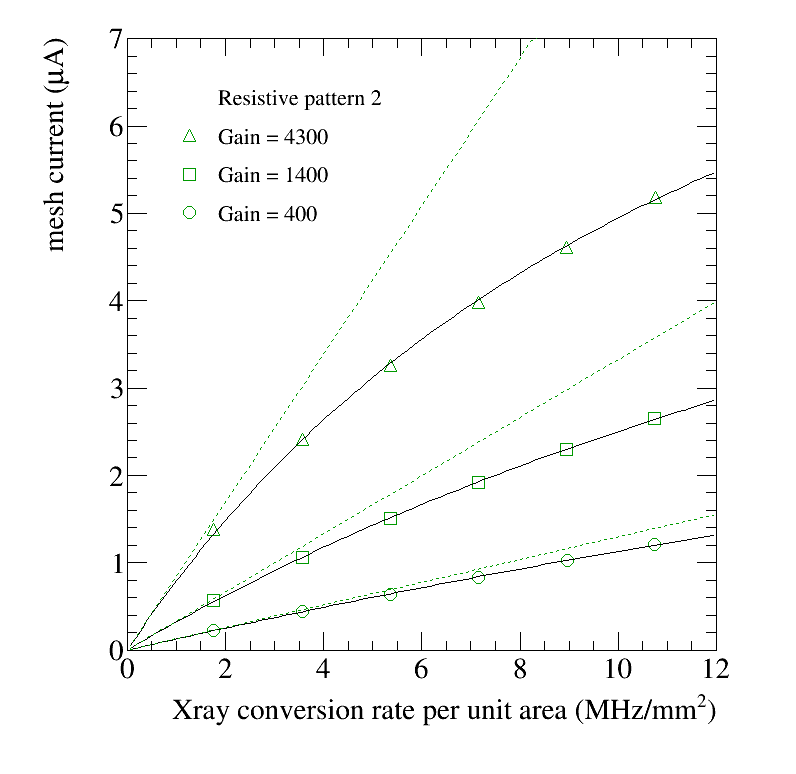
\includegraphics[width=0.45\textwidth]{imesh_rate_mirror}
\caption{Rate capability of resistive prototypes with different embedded resistor patterns (left: lower resistance, right: higher resistance). Dashed lines indicate the non-resistive theorical response. Gain values quoted in the legends are measured at rate sufficiently low that charge-up effects are negligible.}
\label{rateCapa}
\end{centering}
\end{figure}




\subsubsection{Sparking}

Spark suppression was studied using a high-intensity beam of \unit{150}{GeV} pions in the RD51 H4 beam-line of the CERN SPS facility.
The beam was directed at a \unit{2}{\lambda_{\rm int}} deep block of iron.
The prototypes were successively placed \unit{1-2}{mm} downstream of the block and traversed by the hadronic showers.
For each prototype, the mesh current was recorded during couple of spills at a beam intensity reaching up to \unit{1.5}{MHz/cm^{2}}.
Current values during spills are plotted in Figure\,\ref{sparking_RCscan} for all resistive prototypes and one non-resistive prototype.
While the current is relatively constant for most resistive prototypes, strong variations are recorded for the non-resistive prototype. These current variations can be explained by sparking and are also observed for the resistive prototype of shortest RC constant (\unit{1-10}{ns}).
This observation is in line with the spark quenching model presented in section\,\ref{quench_model}.
The latter predicts spark suppression in resistive Micromegas with RC constant larger than the avalanche time-scale of \unit{1-10}{ns}. For shorter time constants, the pad surface voltage decays too fast and the local electric field is restored before the onset of the next avalanche.

\begin{figure}[h]
\centering
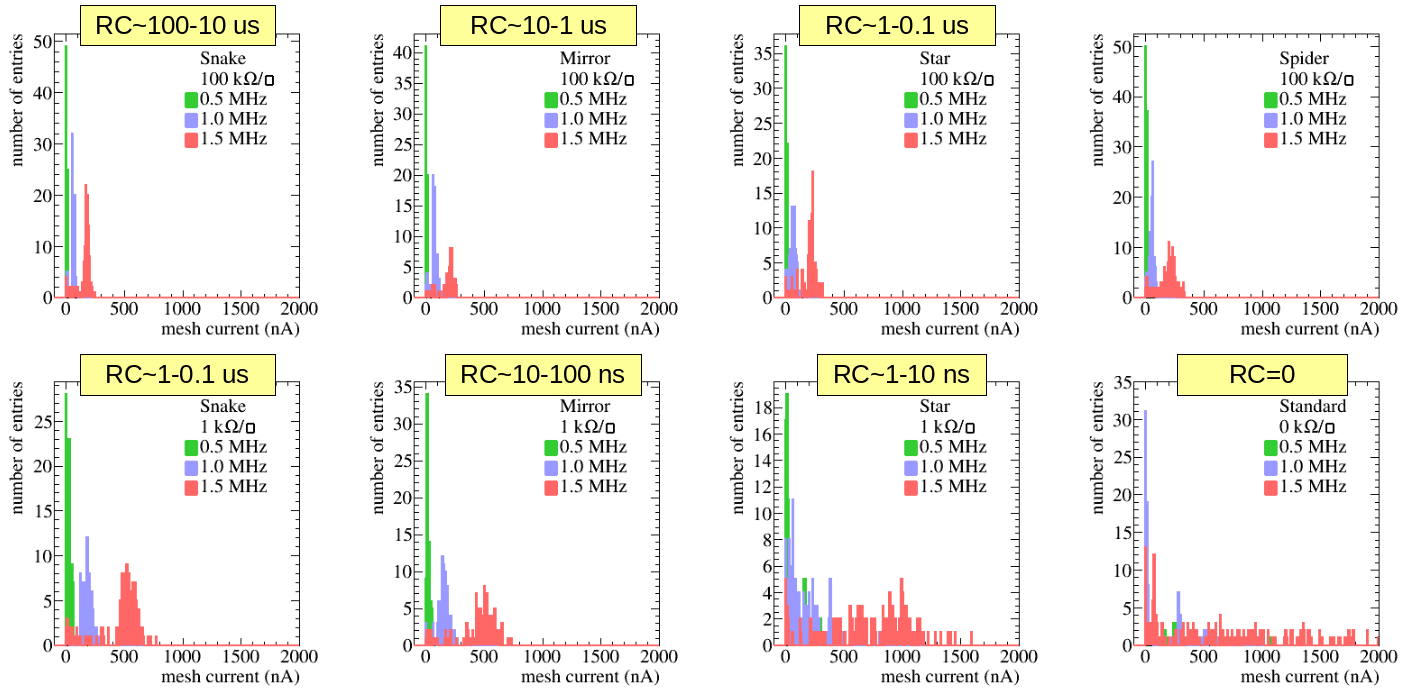
\includegraphics[width=0.95\linewidth]{sparking_RCscan}
\caption{Mesh current of prototypes with different RC constant recorded under high rate of hadron showers. The bottom-right plot was obtained with a non-resistive prototype serving as reference.}
\label{sparking_RCscan}
\end{figure}

\subsection{Future plans}

If correct, the proposed model of spark quenching will allow an optimisation of resistive Micromegas design for full spark suppression and high rate capability. More stringent tests of the model are therefore foreseen; they would use different experimental protocols. After fixing the design of the resistive electrodes, the construction of a small prototype of calorimeter should be pursued. Given available ressources, this prototype will be an electromagnetic calorimeter. It will be used to assess various basic aspects of Micromegas calorimetry such as calibration, temperature effects, linearity and energy resolution. A very first step in this direction was taken during the last testbeam by operating a mini-ECAL composed of a sandwhich of resistive Micromegas and steel absorbers. Event displays of electrons showering into the detector stack are shown in Figure\,\ref{eventDisplay}.


\begin{figure}[h]
\centering
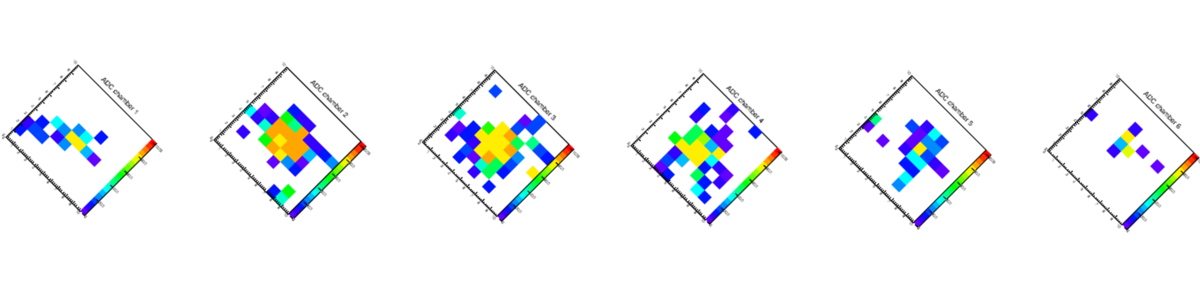
\includegraphics[width=0.95\linewidth]{evtdisplay1}
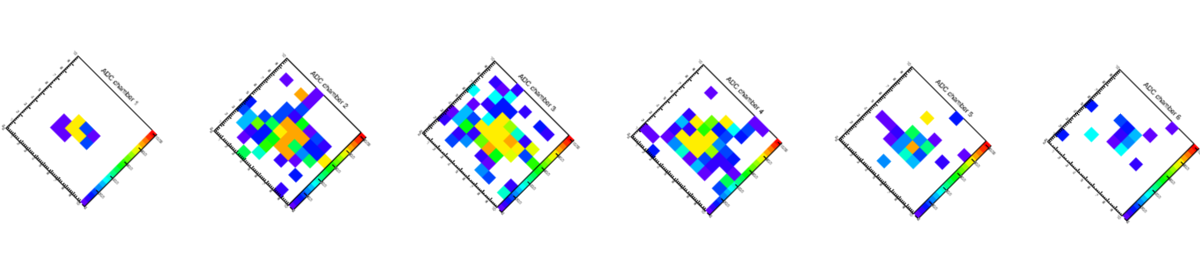
\includegraphics[width=0.95\linewidth]{evtdisplay2}
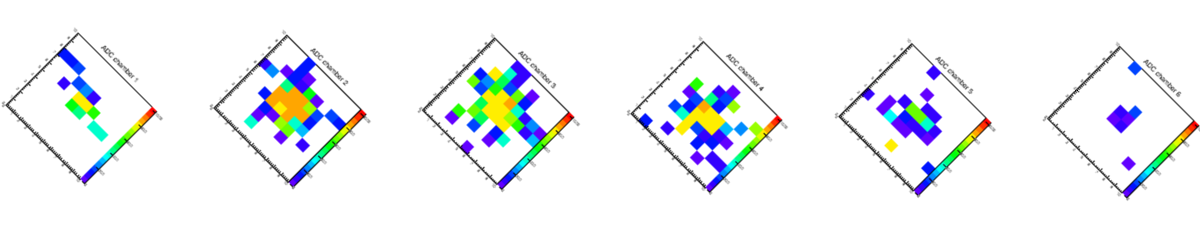
\includegraphics[width=0.95\linewidth]{evtdisplay3}
\caption{From top to bottom: event displays of \unit{200}{GeV} electrons showering in a mini-ECAL of \unit{20}{X_{0}}, composed of 6 resistive Micromegas and steel absorbers. The beam direction is from left to right, the prototype transverse area is 10$\times$\unit{10}{cm^{2}}.}
\label{eventDisplay}
\end{figure}


\end{document}

